%% =====================================================================
%% Overlapping, Not Approximating -- IEEE conference version (IEEEtran)
%% Build:  pdflatex main && bibtex main && pdflatex main && pdflatex main
%% Figures: python make_figures_ieee.py  (writes figures/*.pdf)
%% Items requiring author confirmation before submission are listed in
%% REVIEW_REPORT.md (Section 2).
%% =====================================================================
\documentclass[conference]{IEEEtran}
\IEEEoverridecommandlockouts
\usepackage{cite}
\usepackage{amsmath,amssymb,amsfonts}
\usepackage{graphicx}
\usepackage{booktabs}
\usepackage{array}
\usepackage[table]{xcolor}
\usepackage{tikz}
\usetikzlibrary{patterns,arrows.meta}
\usepackage[hyphens]{url}
\usepackage[hidelinks]{hyperref}
\usepackage{microtype}

\newcommand{\brkus}{\textunderscore\allowbreak}
\newcommand{\code}[1]{{\small\ttfamily\let\_\brkus\hyphenchar\font=-1 #1}}
\newcolumntype{L}[1]{>{\raggedright\arraybackslash}p{#1}}
\newcolumntype{C}[1]{>{\centering\arraybackslash}p{#1}}
\newcommand{\x}{\ensuremath{\times}}
% Table helpers: code at table size (not enlarged), striped rows, roomier rows, group headers.
\newcommand{\tcode}[1]{{\ttfamily\let\_\brkus\hyphenchar\font=-1 #1}}
\definecolor{stripe}{gray}{0.93}
\definecolor{grouphead}{gray}{0.82}
\newcommand{\tablestyle}{\footnotesize\renewcommand{\arraystretch}{1.3}\rowcolors{2}{stripe}{white}}
\newcommand{\group}[2]{\rowcolor{grouphead}\multicolumn{#1}{@{}l}{\textbf{#2}}\\}

\begin{document}

\title{Speeding Up LLM Reinforcement Learning with Idle GPU Time: An Independent Code Audit of TLT}

\author{\IEEEauthorblockN{Eric Hibbs}
\IEEEauthorblockA{Independent Researcher\\
Atlanta, GA, USA\\
ericbhibbs@gmail.com}}

\maketitle

\begin{abstract}
Training a reasoning large language model (LLM) with reinforcement learning (RL) is slow because of one stage: rollout, in which the model writes many candidate answers. Rollout takes roughly 85\% of each training step, and a few very long answers set its pace while many GPUs sit idle. TLT (ASPLOS~'26) uses that idle time to train a small draft model, then uses the draft model to speed up the remaining long answers with speculative decoding. It reports 1.7--2.1\x{} faster training than the VeRL framework without changing the learning algorithm. We checked how those gains arise. We traced eleven mechanisms described in the TLT paper to specific lines of its released code and found five places where the code differs from the paper. The most important is that the online draft-model training ships switched off. We then ran a small test of that training code. Under the pinned software versions, its training pass lets each token see later tokens and other examples packed into the same sequence, which a correct model must not do. We re-checked every reported number against the original paper. Using Amdahl's law, we show that the reported end-to-end gains imply a 1.9--2.6\x{} rollout speedup, which matches the rollout speedups measured directly. We turn the findings into deployment guidance. Scripts that re-run every number check, every code citation, and the test are publicly released.
\end{abstract}

\begin{IEEEkeywords}
Reinforcement learning, large language models, speculative decoding, distributed training systems, GPU utilization, reproducibility.
\end{IEEEkeywords}

%% =====================================================================
\section{Introduction}
\label{sec:intro}

Most of the time spent training a reasoning model with RL goes into one stage, and that stage is slow because of a few very long answers. RL with automatically checked rewards is now the standard way to teach LLMs to reason~\cite{shao2024deepseekmath,deepseekr1}. Each training step starts with \emph{rollout}: the model writes many candidate answers, one token at a time. Hu~\emph{et~al.} measured rollout at approximately 85\% of total step time~\cite[Sec.~1, Fig.~1a]{hu2026tlt}. A batch of answers finishes only when its longest answer finishes. Answer lengths are heavy-tailed: most answers end early, and a few run close to the length limit. While those few finish, many GPUs wait.

A production trace from ByteDance shows the cost. Training Qwen2.5-32B on 128 H20 GPUs took 11~days for only 385 RL steps, approximately 40~min per step~\cite[Sec.~1, Fig.~2]{hu2026tlt}. Throughout the run, the gap between the longest answer and the 75th-percentile answer formed a persistent ``under-utilized zone''~\cite[Fig.~2]{hu2026tlt}. That run used $128 \times 11~\text{days} \times 24~\text{h} = 33{,}792$ GPU-hours. Several other industrial and academic groups report the same long-tail pattern~\cite[Sec.~1]{hu2026tlt}.

There are two ways to speed up a step that waits on a few slow answers. One is to \emph{approximate}: cut slow answers short, or train on answers written by an older version of the model, as fully asynchronous RL systems do~\cite{fu2025areal,zhou2025april}. This uses GPUs better but changes the learning algorithm. The other is to \emph{overlap}: keep the algorithm exactly the same and fill the idle time with useful side work. TLT~\cite{hu2026tlt} takes the second route. While GPUs wait, it trains a small \emph{draft model}, or \emph{drafter}. Once only a few answers are still running, it uses the drafter for speculative decoding (SD)~\cite{leviathan2023,chen2023}, a way to generate text faster without changing the output (Sec.~\ref{sec:background}). TLT therefore speeds up training without changing what the model learns.

This paper is an independent analysis of TLT, not a new system. All experimental results we discuss belong to the TLT authors~\cite{hu2026tlt}. We ask four questions. Which mechanisms produce the speedup? Does the released code implement them as described? Do the reported numbers agree with each other? What must an engineering team do to get the same gains? Our contributions are:
\begin{enumerate}
\item \textbf{A code audit.} We traced eleven mechanisms to specific files and lines of the released \code{fastrl} code~\cite{fastrl} (commit \code{bce3df7}). Five details differ from the paper. Most importantly, online drafter training ships switched off (Sec.~\ref{sec:audit}).
\item \textbf{A test of the drafter-training code.} We ran the released drafter the way the trainer calls it. Under the pinned \code{transformers} version, each token can see later tokens and other packed examples. A control run on the standard model behaves correctly (Sec.~\ref{sec:audit}).
\item \textbf{A checked set of results.} We re-copied every reported number from the source, recomputed every derived number, and recorded the model, hardware, batch size, and decoding settings behind each result (Sec.~\ref{sec:eval}).
\item \textbf{Simple models with stated assumptions.} We use simple math models to explain the size and limits of the speedup. We state where each assumption fails, correct a numerical error in the author's earlier companion model, and use Amdahl's law to check that rollout-level and end-to-end numbers agree (Secs.~\ref{sec:tail} and~\ref{sec:model}).
\item \textbf{Two kinds of ``asynchronous'' speedup, kept apart.} Overlapping side work keeps training exact (lossless). Training on older answers does not (it is off-policy) (Sec.~\ref{sec:async}).
\item \textbf{Deployment guidance:} when the approach pays off, what to configure, what it costs, and what to monitor (Sec.~\ref{sec:practice}).
\end{enumerate}

%% =====================================================================
\section{Background}
\label{sec:background}

\subsection{One Training Step in GRPO}
Each training step has three stages, and only the first is slow. TLT trains with Group Relative Policy Optimization (GRPO)~\cite{shao2024deepseekmath}. GRPO is a variant of Proximal Policy Optimization~\cite{schulman2017ppo} that drops the separately learned critic and instead scores each answer against the other answers to the same prompt. The three stages are~\cite[Sec.~2.1, Fig.~4]{hu2026tlt}:
\begin{enumerate}
\item \emph{Rollout.} The model being trained, called the \emph{policy}, writes several answers per prompt. The released scripts use eight.
\item \emph{Inference.} The policy and a frozen copy of the starting model, the \emph{reference model}, both read the answers. Their outputs give a Kullback--Leibler (KL) penalty, which measures how far the policy has moved from the reference model. A rule-based reward, such as whether the answer is correct, is also computed. In the released setup the KL term is part of the loss (\code{low\_var\_kl}, coefficient 0.001), not part of the reward.
\item \emph{Training.} The policy's weights are updated.
\end{enumerate}
Rollout is slow because it produces one token at a time and must wait for the slowest answer. Inference and training process whole batches at once and run more evenly. TLT adds its side work at the end of rollout. It also reuses the \emph{hidden states}, the model's internal representations of each token, that the inference stage has already computed.

\subsection{Speculative Decoding}
Speculative decoding (SD) speeds up text generation by letting a small model guess and a large model check~\cite{leviathan2023,chen2023}. The small \emph{drafter} guesses the next several tokens. The large \emph{target} model checks all of them in a single pass. It keeps the longest run of guesses it agrees with, plus one token of its own. An analogy: a junior writer drafts the next few words, and a senior editor keeps as many as they would have written themselves. The number of tokens kept per check is the \emph{accept length}.

SD suits RL for two reasons. First, it is \emph{lossless} at the token level. The checking rule guarantees that answers follow exactly the same probability distribution as ordinary generation from the target. This guarantee is about what the answers look like; it says nothing about how fast training converges. Second, SD makes better use of the GPU when few answers are running. Generating one token for a few answers is limited by how fast the GPU can read the model's weights from memory, not by arithmetic. We call this \emph{memory-bandwidth-bound}. Checking many draft tokens at once does more arithmetic per weight read. TLT's roofline analysis~\cite{williams2009roofline}, a standard chart of memory and compute limits, shows SD reaching peak throughput at far smaller batch sizes than normal generation~\cite[Sec.~2.2, Fig.~5c]{hu2026tlt}. So SD helps most in the tail, when few answers are still running.

Using SD inside RL raises three problems~\cite[Sec.~2.2]{hu2026tlt}. (C1)~The target model changes every step, so a fixed drafter goes stale. (C2)~Training a drafter costs GPU time. (C3)~The number of running answers keeps changing, and SD that helps with one answer can slow things down, or run out of memory, with many. TLT's Adaptive Drafter solves C1 and C2. Its Adaptive Rollout Engine solves C3.

\subsection{Two Meanings of ``Asynchronous''}
\label{sec:twoasync}
``Asynchronous'' means two different things in RL systems, and TLT uses only the safe one. In systems such as AReaL~\cite{fu2025areal}, it means the model learns from answers written by an \emph{earlier} version of itself. Generation and training then run at the same time, but training becomes \emph{off-policy}: the model learns from data it did not produce in its current form. In TLT, the learning itself does not change. Each update uses only answers from the current model, so training stays \emph{on-policy}. What runs at the same time is side work: drafter training and saving checkpoints. Neither feeds into the policy update. TLT states this as a design rule it calls the ``Lossless Guarantee''~\cite[Sec.~3]{hu2026tlt}. So every speedup discussed below must come from overlapping side work, never from changing the core update.

%% =====================================================================
\section{Analysis Methodology}
\label{sec:method}

\textbf{Sources.} We used three sources: the TLT paper (arXiv:2511.16665v2)~\cite{hu2026tlt}; the released \code{fastrl} code~\cite{fastrl} at commit \code{bce3df7}, which includes a modified copy of the SGLang~\cite{zheng2024sglang} text-generation engine; and the math (``Model Math'') sections of an earlier interactive dashboard by the author~\cite{hibbs2026dashboard}.

\textbf{Four kinds of claims.} Each statement in this paper is one of four kinds, and we say which kind where it appears.
\emph{Measured:} reported by Hu~\emph{et~al.} and cited by figure or table, as in \cite[Fig./Table]{hu2026tlt}.
\emph{Code-confirmed:} checked in the released code and cited by file and line.
\emph{Modeled:} taken from a simplified math model with stated assumptions; never presented as a measurement.
\emph{Derived:} our own arithmetic or reasoning from cited inputs.

\textbf{How we checked.} (1)~We copied all numbers from the tables and labeled figure values of the arXiv~v2 PDF. We did not use values that could only be estimated from the shape of a plot. (2)~We recomputed every ratio, percentage, and geometric mean in Python. (3)~We re-derived each math model by hand. We also checked the result of Sec.~\ref{sec:tail} with a Monte~Carlo simulation, that is, by averaging over randomly generated batches ($2\times10^5$ batches, fixed random seed). (4)~We traced each mechanism to the code by reading the relevant classes, configuration files, and launch scripts. (5)~When reading the code suggested a bug, we ran the released code to test it (Sec.~\ref{sec:audit}).

\textbf{Reproducibility package.} Three scripts come with the paper~\cite{hibbs2026artifact}. \code{verify\_numbers.py} recomputes all 44 derived numbers in this paper from their stated inputs and checks them against the printed values. \code{verify\_code\_claims.py} checks all 41 code citations against \code{fastrl} at \code{bce3df7}. \code{test\_drafter\_masking.py} is the test described in Sec.~\ref{sec:audit}. At submission, all checks pass, and the test gives the results reported there.

\textbf{What is original here.} The measurements belong to Hu~\emph{et~al.} Our own contributions are the code audit and the differences it found, the masking test, the corrections and consistency checks of reported and modeled numbers, the Amdahl analysis, the comparison of asynchronous approaches in Sec.~\ref{sec:async}, and the deployment guidance. The math models in Secs.~\ref{sec:tail} and~\ref{sec:model} come from the author's earlier dashboard~\cite{hibbs2026dashboard}. We reuse them with their assumptions stated and one error corrected.

%% =====================================================================
\section{Why a Few Long Answers Slow Everything Down}
\label{sec:tail}

A batch finishes only when its slowest answer finishes. Let a batch hold $B$ answers with token lengths $L_1,\dots,L_B$, each generated at $r_i$ tokens per second. Then the time for the batch is
\begin{equation}
T_{\text{batch}} = \max_{i\le B} \frac{L_i}{r_i}.
\label{eq:tbatch}
\end{equation}
In statistics, the largest value in a sample is an \emph{order statistic}. To see how the slowest answer grows with batch size, the companion model~\cite{hibbs2026dashboard} assumes that the lengths are independent draws from a Pareto distribution, $P(L>x)=(x_{\min}/x)^{\alpha}$ with $\alpha>1$. The Pareto distribution is a standard model of heavy tails: most values are small, but very large values are not rare. A smaller $\alpha$ means a heavier tail. This is an assumption. TLT's measured lengths have a shape closer to log-normal~\cite[Fig.~1a]{hu2026tlt}. Under the assumption, the expected length of the longest answer is
\begin{equation}
\begin{split}
\mathbb{E}[M_B] &= x_{\min}\,\frac{\Gamma(B+1)\,\Gamma(1-1/\alpha)}{\Gamma(B+1-1/\alpha)}\\
&\approx x_{\min}\,B^{1/\alpha}\,\Gamma(1-1/\alpha),
\end{split}
\label{eq:emax}
\end{equation}
where the approximation uses $\Gamma(B+1)/\Gamma(B+1-1/\alpha)\sim B^{1/\alpha}$. So the longest answer grows like $B^{1/\alpha}$. The heavier the tail, the faster the worst case grows with batch size, and the more GPU time sits idle while it runs.

\textbf{Worked example and a correction (derived).} With $\alpha=2$ and $B=128$, Eq.~(\ref{eq:emax}) gives $\mathbb{E}[M_B]=20.07\,x_{\min}$. A Monte~Carlo simulation ($2\times10^5$ batches) gives $20.12\,x_{\min}$. Under this model the median answer is $2^{1/\alpha}x_{\min}=1.414\,x_{\min}$. So the expected longest answer is about $14.2\times$ the median answer. The author's earlier dashboard used a different formula. It replaced the factor $\Gamma(1-1/\alpha)=\sqrt{\pi}\approx1.77$ with the Pareto mean factor $\alpha/(\alpha-1)=2$, which gives $22.63\,x_{\min}$ (16.0\x{} the median). The dashboard also stated a ratio of ``$\approx5.7\times$''. That number equals $B^{1/\alpha}/\alpha=\sqrt{128}/2=5.66$, which results from a normalization error. The value of about $14.2\times$ above replaces it.

\textbf{Link to the measurements.} Real answers are also cut off at the generation limit: 20,480 tokens in the ByteDance trace and 32K tokens in TLT's experiments. The measured longest answer reaches that limit again and again~\cite[Fig.~2]{hu2026tlt}. The model and the trace agree on the point that matters for system design: idle GPU time is built into the workload, not occasional. It lasts across all 385 steps of the production run. That is why TLT \emph{uses} the idle time rather than only trying to shorten it.

%% =====================================================================
\section{How TLT Uses the Idle Time}
\label{sec:design}

TLT combines several mechanisms that fill idle GPU time or hide costs. Fig.~\ref{fig:timeline} contrasts a normal rollout with TLT's overlapped one. Table~\ref{tab:mech} lists each mechanism, the cost it hides, its measured effect, and where it is in the released code.

\begin{figure}[t]
\centering
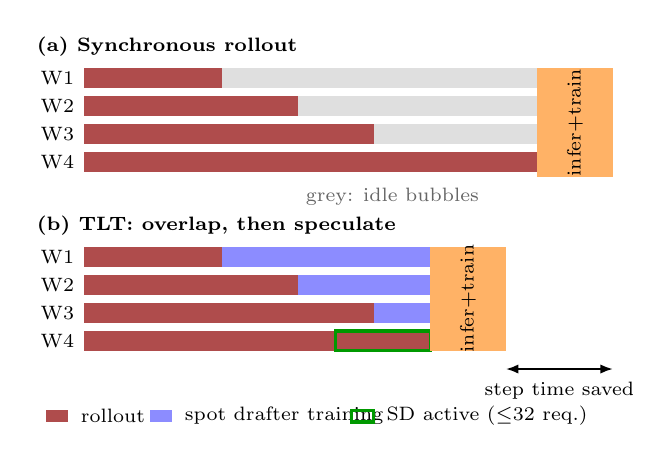
\begin{tikzpicture}[x=0.80cm,y=0.42cm,font=\scriptsize]
  % ---------- (a) synchronous baseline
  \node[anchor=west] at (-0.9,9.0) {\textbf{(a) Synchronous rollout}};
  \foreach \w/\e [count=\i] in {1/2.2,2/3.4,3/4.6,4/7.2}{
    \pgfmathsetmacro{\yy}{8.6-\i*0.85}
    \node[anchor=east] at (0,\yy+0.3) {W\w};
    \fill[red!55!black!70] (0,\yy) rectangle (\e,\yy+0.6);
    \ifnum\i<4 \fill[gray!25] (\e,\yy) rectangle (7.2,\yy+0.6); \fi
  }
  \fill[orange!60] (7.2,5.05) rectangle (8.4,8.35);
  \node[rotate=90] at (7.8,6.7) {infer+train};
  \node at (4.9,4.45) {\textcolor{gray!80!black}{grey: idle bubbles}};
  % ---------- (b) TLT
  \node[anchor=west] at (-0.9,3.6) {\textbf{(b) TLT: overlap, then speculate}};
  \foreach \w/\e [count=\i] in {1/2.2,2/3.4,3/4.6,4/5.5}{
    \pgfmathsetmacro{\yy}{3.2-\i*0.85}
    \node[anchor=east] at (0,\yy+0.3) {W\w};
    \fill[red!55!black!70] (0,\yy) rectangle (\e,\yy+0.6);
    \ifnum\i<4 \fill[blue!45] (\e,\yy) rectangle (5.5,\yy+0.6); \fi
  }
  \draw[green!60!black,very thick] (4.0,-0.20) rectangle (5.5,0.40);
  \fill[orange!60] (5.5,-0.20) rectangle (6.7,2.95);
  \node[rotate=90] at (6.1,1.38) {infer+train};
  \draw[{Latex[length=1.6mm]}-{Latex[length=1.6mm]},thick] (6.7,-0.75) -- (8.4,-0.75);
  \node[anchor=north] at (7.55,-0.85) {step time saved};
  % ---------- legend
  \fill[red!55!black!70] (-0.6,-2.35) rectangle (-0.25,-2.0); \node[anchor=west] at (-0.2,-2.17) {rollout};
  \fill[blue!45] (1.05,-2.35) rectangle (1.4,-2.0); \node[anchor=west] at (1.45,-2.17) {spot drafter training};
  \draw[green!60!black,very thick] (4.25,-2.35) rectangle (4.6,-2.0); \node[anchor=west] at (4.65,-2.17) {SD active ($\le$32 req.)};
\end{tikzpicture}
\caption{One RL step on four rollout workers (W1--W4), drawn to show the idea, not to scale. (a)~Workers that finish early sit idle until the longest answer completes. (b)~TLT trains the drafter on the freed workers without holding up rollout, and turns on speculative decoding once few answers remain, which shortens the tail. Adapted from the illustration in~\cite[Fig.~1b]{hu2026tlt}.}
\label{fig:timeline}
\end{figure}

\begin{table*}[t]
\centering
\caption{TLT's Mechanisms: The Cost Each Hides, Its Measured Effect, and Where It Is in the Code}
\label{tab:mech}
\tablestyle
\begin{tabular}{@{}L{2.75cm}L{3.0cm}L{3.15cm}L{1.25cm}L{6.15cm}@{}}
\toprule
\rowcolor{white}\textbf{Mechanism} & \textbf{Cost it overlaps or hides} & \textbf{Measured effect} & \textbf{TLT ref.} & \textbf{Code location} (file\,:\,lines) \\
\midrule
Spot Trainer (non-blocking drafter training) & Drafter training, moved into rollout bubbles & Drafter cost hidden in the bubble & Abstr., 4.2 & \tcode{eagle\_background\_trainer.py}\,:\,35 \\
DataBuffer with one-step offset & Bias toward short, early-finishing sequences & Partial + buffered data $\approx$ full-set training & Sec.~4.2 & \tcode{worker\_manager.py}\,:\,489--493\newline \tcode{eagle\_background\_trainer.py}\,:\,276--302 \\
Worker Coordinator (state machine) & Contention between drafter work and rollout & Stage transition $<$1\% of step & Sec.~6.4 & \tcode{worker\_manager.py}\,:\,54--61 \\
Selective async checkpointing & Checkpoint I/O stalls & 893\,$\to$\,280\,$\to$\,97\,ms (9.2\x) & Fig.~17a & \tcode{eagle\_background\_trainer.py}\,:\,83, 119--148 \\
Single-layer drafter & Drafter latency and training cost & 2.4\x{} faster than a 0.5B drafter & Sec.~4.1 & \tcode{eagle\_trainer.py}\,:\,190, 256--258 \\
Sequence packing & Padding waste in drafter training & 13.3\,$\to$\,29.6 samples/s (2.2\x) & Fig.~17b & \tcode{eagle\_background\_trainer.py}\,:\,410--417 \\
Adaptive SD activation & SD overhead at large batch sizes & 2.44\x{} rollout case study & Fig.~14 & \tcode{eagle\_worker.py}\,:\,196, 361--364 \\
Tree drafting & Low acceptance of single-path drafts & 3.66\x{} peak SD speedup & Fig.~13b & \tcode{eagle\_worker.py}\,:\,748--821 \\
Bucketed CUDAGraph & Graph memory for many SD strategies & 30.39\,$\to$\,10.69\,GB (2.8\x) & Table~5 & \tcode{server\_args.py}\,:\,789--796 \\
BEG-MAB strategy tuner & Manual SD hyperparameter tuning & Strategy chosen per batch size & Sec.~6.3 & \tcode{eagle\_mab.py}\,:\,197--292\newline \tcode{eagle\_worker.py}\,:\,1234--1240 (reward) \\
Model-free $n$-gram drafter & No learned drafter early in training & Fallback keeps SD available & Sec.~5.3 & \tcode{ngram\_worker.py}\newline \tcode{server\_args.py}\,:\,342--346 \\
\bottomrule
\end{tabular}
\vspace{3pt}

\raggedright\footnotesize Measured effects are from Hu \emph{et al.}~\cite{hu2026tlt}; code locations are in \code{fastrl} at commit \code{bce3df7}. Directories: \tcode{eagle\_background\_trainer.py} is in \tcode{verl/workers/drafter/}; \tcode{worker\_manager.py} in \tcode{verl/workers/rollout/sglang\_rollout/}; \tcode{eagle\_trainer.py} in \tcode{eagle-train/}; \tcode{server\_args.py} in \tcode{third-party/sglang/python/sglang/srt/}; and \tcode{eagle\_worker.py}, \tcode{eagle\_mab.py}, \tcode{ngram\_worker.py} in that directory's \tcode{speculative/} subfolder.
\end{table*}

\subsection{Training the Drafter Without Holding Up Rollout}
TLT trains the drafter during the tail instead of adding a fourth stage after rollout. A simple design would add that fourth stage~\cite[Fig.~8]{hu2026tlt}. TLT's Spot Trainer (class \code{EagleBackgroundTrainer}) instead starts training as soon as enough short answers have finished, using these \emph{partial} results, and runs in a non-blocking manner during the tail~\cite[Sec.~4.2]{hu2026tlt}. Training only on the answers that finish first would bias the drafter toward short answers. So a DataBuffer stores hidden states and tokens from the inference stage and mixes data across steps, running one step behind. In the code, data are collected on the step \emph{before} each training step (\code{(step+1) \% interval == 0}), and each training batch is drawn from the last two RL steps (\code{buffer\_steps = 2}). Because the hidden states are reused from the inference stage, drafter training needs no extra pass through the target model. The target model is over 20\x{} larger than the drafter~\cite[Sec.~4.1]{hu2026tlt}.

\subsection{Scheduling Side Work So It Can Always Be Interrupted}
A central coordinator decides which GPUs may train the drafter and stops that work the moment rollout ends. It runs on the first process (rank~0) and uses the ZeroMQ messaging library. It tracks each rollout \emph{worker}, which is one copy of the model being served. For example, one copy split across eight GPUs counts as one worker; we write this as TP\,=\,8, where TP (tensor parallelism) is the number of GPUs one model copy is split across. The paper describes each worker as moving through three states: BUSY, IDLE, TRAINING~\cite[Sec.~4.2]{hu2026tlt}. The code uses five: \code{IDLE}, \code{GENERATING}, \code{RELEASED}, \code{TRAINING}, and \code{COMPLETED}. Workers that have released their GPUs start drafter training once at least \code{min\_workers\_for\_training} of them are free (default~1). When rollout ends, the coordinator broadcasts \code{STOP\_TRAINING} and \code{BATCH\_COMPLETE} messages. Drafter training therefore acts as a low-priority ``spot'' task that never delays the RL step. The shipped setting trains the drafter every ten steps (\code{training\_interval\_steps: 10}), matching the paper's finding that this is enough~\cite[Sec.~6.4]{hu2026tlt}.

\subsection{Saving Checkpoints in the Background}
Because drafter training can be interrupted at any time, it must save checkpoints often, and saving would itself stall training. TLT saves in a background thread with PyTorch Distributed Checkpoint (\code{dcp.async\_save}). It also skips two frozen weight tensors, \code{model.embed\_tokens.weight} and \code{lm\_head.weight}. These belong to the \emph{embedding} and the \emph{LM head}, the layers that convert between tokens and the model's internal vectors. Measured save time falls from 893\,ms (normal) to 280\,ms (in the background, 3.2\x) to 97\,ms (in the background and skipping frozen weights, 9.2\x{} faster than normal)~\cite[Fig.~17a]{hu2026tlt}. The 9.2\x{} is a measured time, not a ratio of parameter counts. Saving in the background gives the first 3.2\x{}. Skipping the frozen embedding and LM head, which make up most of a one-layer drafter's parameters, gives the remaining 2.9\x{} (derived).

\subsection{A One-Layer Drafter and Packed Training Data}
The drafter is a single trainable transformer layer (\code{num\_hidden\_layers = 1}). It reuses the target model's frozen embedding and LM head, so only about $1/\text{num\_layers}$ of the target's parameters are trained~\cite[Sec.~4.1]{hu2026tlt}. The paper argues that a drafter's speed depends mostly on how many layers it has. A Qwen2.5-0.5B drafter has 24 layers, and TLT's one-layer drafter of similar parameter count is 2.4\x{} faster~\cite[Sec.~4.1]{hu2026tlt}. In the code, the drafter's loss combines a Smooth-L1 (Huber) loss on hidden states with a soft-target cross-entropy loss on predicted tokens, weighted 0.5 each. This is a more specific form of the paper's ``L1\,+\,CE.'' To avoid wasting compute on padding, \emph{sequence packing}~\cite{krell2021packing} joins training examples of different lengths into one long sequence. This raises drafter-training throughput from 13.3 to 29.6 samples/s (2.2\x)~\cite[Fig.~17b]{hu2026tlt}. Sec.~\ref{sec:masktest} tests how the code keeps packed examples apart.

\subsection{Turning Speculative Decoding On at the Right Time}
TLT turns SD on only when the number of answers still running falls to a threshold (default~32)~\cite[Sec.~5.1]{hu2026tlt}. The code adds a safeguard that the paper does not describe. SD turns on only after the count has stayed at or below 32 for ten checks in a row (\code{adaptive\_spec\_warmup\_checks = 10}). This \emph{hysteresis} stops SD from flickering on and off. The drafter guesses in a tree. It explores the \code{topK} most likely tokens at each of \code{Draft\_Depth} steps, and the target checks the \code{Tokens\_to\_Verify} most promising guesses in one pass~\cite[Sec.~5.1, Fig.~9]{hu2026tlt}.

Each SD setting needs its own \emph{CUDA graph}, a pre-recorded sequence of GPU operations that runs faster than issuing them one at a time. Recording a separate graph for every setting uses a lot of memory. TLT's bucketed CUDAGraph capture groups batch sizes into buckets, records drafter and target graphs separately, and shares identical ones. For Llama-3-8B (TP\,=\,4, four settings), graph memory is 7.81\,GB for one setting, 30.39\,GB when recording each setting separately, and 10.69\,GB with buckets. That is 2.8\x{} less than separate recording, at 1.37\x{} the memory of a single setting~\cite[Table~5]{hu2026tlt}.

A learning algorithm picks the SD setting automatically. TLT uses a bucketed epsilon-greedy multi-armed bandit (BEG-MAB): it usually picks the setting that has worked best so far and occasionally tries another~\cite[Sec.~5.2, Alg.~1]{hu2026tlt}. Each option is a $(\text{Draft\_Depth}, \text{topK}, \text{Tokens\_to\_Verify})$ combination. The code confirms the reward. With mean tokens kept per answer $a=\sum_i \text{accept\_len}_i/B + 1$, the reward is $a\,B/t_{\text{elapsed}}$, that is, tokens kept per second. Defaults set in the code but not stated in the paper are an exploration rate $\epsilon=0.1$, a 1000-sample sliding window, batch-size bucket boundaries $\{1,2,5,21\}$, and a memory guard $\text{draft\_tokens}\times B\le 2048$. Before a trained drafter exists, a drafter that needs no training is used instead. It looks up repeated token sequences ($n$-grams) in other answers to the same prompt, in the style of Lookahead~\cite{zhao2024lookahead} (maximum match window~12, branch length~18)~\cite[Sec.~5.3]{hu2026tlt}. In a 128-request rollout of Qwen-32B on H100 GPUs, SD switches on below 32 remaining requests, and rollout finishes in 138\,s instead of 337\,s without SD, a 2.44\x{} speedup~\cite[Fig.~14]{hu2026tlt}.

%% =====================================================================
\section{Simple Models of the Speedup}
\label{sec:model}

The formulas in this section are \emph{modeled}~\cite{hibbs2026dashboard}. They rest on simplifying assumptions and are not fitted to TLT's measurements. We use them only to explain which way the speedup moves and where it levels off, and we compare them with the measurements in~\cite{hu2026tlt}.

\subsection{How Many Tokens SD Keeps per Check}
\label{sec:model-en}
Each extra guessed token helps less than the one before. Assume the drafter guesses $\gamma$ tokens and the target accepts each one independently with probability $\alpha$. Let $A$ be the number of guesses accepted in a row; then $P(A\ge k)=\alpha^{k}$ for $k\le\gamma$. One extra token is always kept, so the expected number of tokens kept per check is
\begin{equation}
\mathbb{E}[n] = \sum_{k=0}^{\gamma}\alpha^{k} = \frac{1-\alpha^{\gamma+1}}{1-\alpha}.
\label{eq:en}
\end{equation}
If every guess is accepted ($\alpha\to1$), $\mathbb{E}[n]\to\gamma+1$. If the drafter guesses without limit ($\gamma\to\infty$), $\mathbb{E}[n]\to1/(1-\alpha)$, for example 5.0 at $\alpha=0.8$. The measurements level off in the same way: accept length flattens as depth grows, reaching 9.78 tokens at Draft\_Depth\,=\,16 and Tokens\_to\_Verify\,=\,128~\cite[Fig.~13a]{hu2026tlt}. The assumption of the same $\alpha$ at every position is false in practice. Measured acceptance drops for guesses further ahead~\cite[Fig.~16]{hu2026tlt}, so the model is qualitative.

\subsection{Why There Is a Best Draft Depth}
\label{sec:model-sp}
Guessing deeper first raises the speedup and then lowers it. Let $c=T_{\text{verify}}/T_{\text{draft}}$, the time for one check divided by the time for one draft step. One cycle costs one check plus $\gamma$ draft steps, or $1+\gamma/c$ check-times. So
\begin{equation}
\text{speedup}(\gamma) = \frac{\mathbb{E}[n]}{1+\gamma/c}.
\label{eq:speedup}
\end{equation}
The tokens kept per check level off as $\gamma$ grows, but the cost keeps growing in a straight line. So the speedup rises, peaks, and falls. At $\alpha=0.8$, the best depth is $\gamma^{*}=3,5,7$ for $c=4,8,16$ (Fig.~\ref{fig:model}a). Cheaper drafting (a larger $c$) favors deeper guesses. The measurements behave the same way. Accept length keeps rising with depth, but speedup peaks at 3.66\x{} at Draft\_Depth\,=\,12 and Tokens\_to\_Verify\,=\,64 and falls after that~\cite[Fig.~13b]{hu2026tlt}. Speedup barely changes with \code{topK} (3.47--3.65\x{} for $\text{topK}\in[4,16]$)~\cite[Table~1]{hu2026tlt}. That is why TLT fixes \code{topK} and tunes only the other two settings. These grids were measured at temperature~0, which gives stable accept lengths; RL rollouts use temperature~0.9.

\begin{figure}[t]
\centering
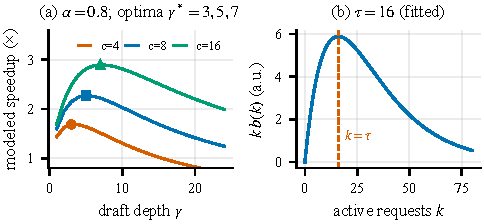
\includegraphics[width=\columnwidth]{figures/fig_model.pdf}
\caption{Modeled, not measured. (a)~Speedup from Eq.~(\ref{eq:speedup}) versus draft depth for three check-to-draft cost ratios $c$, with the same acceptance $\alpha=0.8$ at every position. Markers show the best depth. (b)~Total SD benefit $k\,b(k)$ from Eq.~(\ref{eq:thresh}) with a fitted $\tau=16$; it peaks at $k=\tau$.}
\label{fig:model}
\end{figure}

\subsection{Why SD Should Switch Off for Large Batches}
\label{sec:model-th}
With many answers running, the GPU is already busy with arithmetic, so checking extra draft tokens gains less. The companion model writes the benefit per answer, when $k$ answers are running, as $b(k)=b_0e^{-k/\tau}$. It turns SD on when the total benefit beats the cost of switching, $O_{\text{SD}}$:
\begin{equation}
k\,b(k) = b_0\,k\,e^{-k/\tau} \;\ge\; O_{\text{SD}}.
\label{eq:thresh}
\end{equation}
Since $\frac{d}{dk}\bigl(k e^{-k/\tau}\bigr)=e^{-k/\tau}(1-k/\tau)$, the total benefit peaks at $k=\tau$ and then falls (Fig.~\ref{fig:model}b). This explains why a batch-size threshold \emph{exists}. The value $\tau=16$ was chosen to resemble the measured trend; it is not from the paper. The code also uses a hard cutoff (batch size $\le32$ with the ten-check hysteresis), not this smooth curve. The measurements are in Table~4 of~\cite{hu2026tlt} (Fig.~\ref{fig:batch}). At Tokens\_to\_Verify\,=\,64, SD speedup falls from 3.62\x{} at batch size~1 to 1.70\x{} at batch size~32. At batch size~32, the best setting checks the \emph{fewest} tokens (2.48\x{} at 16). The author's earlier dashboard stated that SD ``drops to 1.08\x{} at BS\,=\,32''; that value does not appear in Table~4 and is not used here.

\begin{figure}[t]
\centering
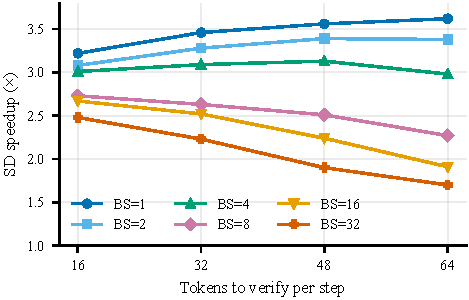
\includegraphics[width=\columnwidth]{figures/fig_batch.pdf}
\caption{Measured SD speedup versus tokens checked per step, for six batch sizes (Qwen2.5-32B, H100, TP\,=\,4, Draft\_Depth\,=\,10, topK\,=\,8). Data from~\cite[Table~4]{hu2026tlt}. Larger batches do best when checking fewer tokens, which is why TLT picks SD settings automatically.}
\label{fig:batch}
\end{figure}

\subsection{Keeping the Drafter Up to Date}
\label{sec:model-drift}
The drafter must keep learning, because the model it imitates changes every step. The drafter minimizes $\mathcal{L}(\theta_t)=\mathbb{E}_{x\sim\pi_t}[-\log p_{\theta_t}(x)]$, where $\pi_t$ is the policy at step $t$. The companion model makes two approximations. First, the Fisher information $I_t$, a measure of how much the drafter can learn from each update, stays roughly constant. Second, acceptance relates to the KL distance between policy and drafter as $\alpha\approx e^{-D_{\mathrm{KL}}}$. It then writes the step-to-step relation
\begin{equation}
D_{\mathrm{KL}}(\pi_{t+1}\Vert p_{\theta_{t+1}}) \le D_{\mathrm{KL}}(\pi_t\Vert p_{\theta_t}) - \eta_d I_t + \delta_\pi + O(\eta_d^2),
\label{eq:drift}
\end{equation}
where $\eta_d$ is the drafter's learning step size and $\delta_\pi$ is how far the policy moves in one step. To first order, acceptance does not fall on average when $\eta_d I_t>\delta_\pi$. In plain words, the drafter keeps up if it learns faster than the policy changes. Inequality~(\ref{eq:drift}) is a rough tracking model built on the two approximations above, not a convergence theorem. We use it only to organize the evidence. Three measurements fit this picture. Drafter top-3 accuracy dips after each policy update and recovers within a few drafter training steps~\cite[Fig.~15]{hu2026tlt}. Training the drafter alongside RL raises accept length from 4.59 to 6.53 on RL rollouts (+42.3\%, derived) and from 3.76 to 5.15 on downstream MT-Bench tasks (+37.0\%, derived)~\cite[Table~6]{hu2026tlt}. And the adaptive drafter keeps higher acceptance for guesses further ahead than a non-adaptive drafter~\cite[Fig.~16]{hu2026tlt}.

\subsection{Do the Reported Speedups Agree?}
\label{sec:amdahl}
The end-to-end and rollout-level speedups that TLT reports are consistent with each other. Amdahl's law~\cite{amdahl1967} says how much a whole job speeds up when only part of it gets faster. If a fraction $f$ of step time is rollout, and only rollout speeds up by a factor $s$, the whole step speeds up by
\begin{equation}
S = \frac{1}{(1-f) + f/s}, \qquad s = \frac{f}{1/S-(1-f)}.
\label{eq:amdahl}
\end{equation}
With the measured $f\approx0.85$~\cite[Fig.~1a]{hu2026tlt}, the most that speeding up rollout could ever achieve is $1/(1-f)\approx6.7\times$. The measured end-to-end speedups range from $S=1.66$ to $2.12\times$ (Sec.~\ref{sec:eval}). Solving Eq.~(\ref{eq:amdahl}) for $s$ gives a rollout speedup of $s\approx1.9$--$2.6\times$ (derived). This is close to the rollout speedups measured directly: 2.44\x{} in the 128-request case study~\cite[Fig.~14]{hu2026tlt} and 2.33--3.22\x{} in batch-size-1 benchmarks~\cite[Table~2]{hu2026tlt} (Fig.~\ref{fig:amdahl}). So the end-to-end and rollout-level numbers agree. The bound also shows how much room is left: even an infinitely fast rollout cannot make the step more than 6.7\x{} faster unless the other 15\% of the step also gets faster. This check assumes that $f$ is the same across the models and clusters tested; the paper reports $f$ for one setup only.

\begin{figure}[t]
\centering
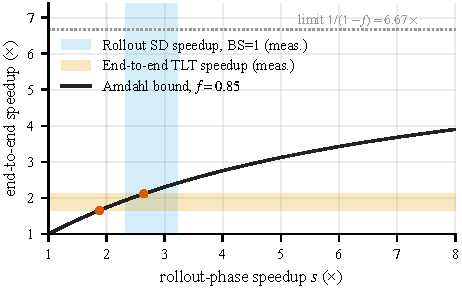
\includegraphics[width=\columnwidth]{figures/fig_amdahl.pdf}
\caption{Amdahl's law, Eq.~(\ref{eq:amdahl}), with rollout fraction $f=0.85$~\cite[Fig.~1a]{hu2026tlt}. Shaded bands: measured end-to-end TLT speedups~\cite[Fig.~11]{hu2026tlt} and measured batch-size-1 rollout SD speedups~\cite[Table~2]{hu2026tlt}. Dots: the rollout speedups implied by the lowest and highest end-to-end results (derived).}
\label{fig:amdahl}
\end{figure}

%% =====================================================================
\section{What TLT Reports}
\label{sec:eval}

\subsection{How the TLT Authors Measured}
TLT reports faster training steps, measured on large GPU clusters with an already-trained drafter. TLT is built on VeRL~\cite{sheng2025hybridflow} and the Ray framework~\cite{moritz2018ray}, with SGLang~\cite{zheng2024sglang} generating the rollouts~\cite[Sec.~6.1]{hu2026tlt}. The main test machine is eight NVIDIA DGX H100 servers, 64 GPUs in total. Each server has eight H100 GPUs, two Intel Xeon Platinum 8480C CPUs, and 2\,TB of memory. GPUs within a server connect at 900\,GB/s (NVLink), and servers connect at 400\,Gb/s (InfiniBand). A separate DGX A100 cluster was also used. The models are Qwen2.5-7B, DeepSeek-R1-Distill-Qwen-7B, Qwen2.5-32B, and Llama-3.3-70B-Instruct. RL uses GRPO with temperature~0.9, a maximum answer length of 32K tokens, TP\,$\in\{2,4,8\}$, the Adam optimizer, and BF16 numbers. The RL data are a subset of Eurus-2-RL~\cite{cui2025prime}, and the drafter is first trained on a subset of OpenThoughts2-1M. The comparison systems are Open-R1~\cite{openr1}, VeRL, and TLT-Base, which is TLT with plain SD and the no-training $n$-gram drafter. The metric is token throughput: all prompt and answer tokens in a batch divided by the time for one RL step. It is averaged over three steps after one warm-up step, using an already-trained drafter~\cite[Sec.~6.1]{hu2026tlt}. So the reported gains are \emph{faster steps with matching reward curves}. They do not mean fewer steps to reach a target reward. Fig.~\ref{fig:e2e} and Tables~\ref{tab:e2e}--\ref{tab:results} collect the reported results and their conditions.

\begin{figure*}[t]
\centering
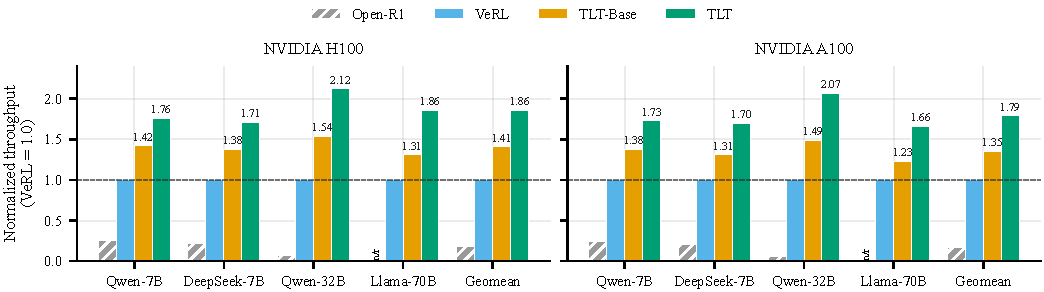
\includegraphics[width=\textwidth]{figures/fig_e2e.pdf}
\caption{End-to-end RL training throughput relative to VeRL (GRPO). Values from~\cite[Fig.~11]{hu2026tlt}; labels shown for TLT-Base and TLT. ``n/r'': no Open-R1 result reported for Llama-70B. The source gives geometric-mean TLT speedups of 1.86\x{} (H100) and 1.79\x{} (A100).}
\label{fig:e2e}
\end{figure*}

\begin{table}[t]
\centering
\caption{End-to-End Speedup over VeRL Reported by Hu \emph{et al.}~\cite{hu2026tlt} (VeRL\,=\,1.00)}
\label{tab:e2e}
\tablestyle
\textbf{(a)} By model and GPU (TLT Fig.~11)\par\vspace{2pt}
\begin{tabular}{@{}L{2.3cm}C{0.95cm}C{1.15cm}C{0.95cm}C{1.15cm}@{}}
\toprule
\rowcolor{white} & \multicolumn{2}{c}{\textbf{H100}} & \multicolumn{2}{c}{\textbf{A100}} \\
\cmidrule(lr){2-3}\cmidrule(l){4-5}
\rowcolor{white}\textbf{Model} & TLT & TLT-Base & TLT & TLT-Base \\
\midrule
Qwen2.5-7B & 1.76 & 1.42 & 1.73 & 1.38 \\
DeepSeek-R1-7B & 1.71 & 1.38 & 1.70 & 1.31 \\
Qwen2.5-32B & 2.12 & 1.54 & 2.07 & 1.49 \\
Llama-3.3-70B & 1.86 & 1.31 & 1.66 & 1.23 \\
\midrule
\rowcolor{white}\textbf{Geomean} & \textbf{1.86} & 1.41 & \textbf{1.79}$^{*}$ & 1.35 \\
\bottomrule
\end{tabular}

\vspace{6pt}
\textbf{(b)} By cluster size, TLT only (TLT Table~3)\par\vspace{2pt}
\begin{tabular}{@{}L{2.3cm}C{1.05cm}C{1.05cm}C{1.05cm}C{1.05cm}@{}}
\toprule
\rowcolor{white}\textbf{Model} & 1 node & 2 nodes & 4 nodes & 8 nodes \\
\midrule
Qwen2.5-7B & 1.21 & 1.45 & 1.62 & 1.76 \\
Qwen2.5-32B & OOM & OOM & 1.83 & 2.12 \\
\bottomrule
\end{tabular}
\vspace{3pt}

\raggedright\footnotesize Nodes have 8 GPUs each; OOM = out of memory. Open-R1 reaches 0.06--0.25\x{} of VeRL where reported. $^{*}$As printed in the source; the geometric mean of the rounded per-model values is 1.78.
\end{table}

\begin{table}[t]
\centering
\caption{Rollout Speedup from Speculative Decoding Across GPUs (Qwen2.5-7B, BS\,=\,1, TP\,=\,1; TLT Table~2)}
\label{tab:gpu}
\tablestyle
\begin{tabular}{@{}L{1.6cm}C{1.9cm}C{1.9cm}C{1.4cm}@{}}
\toprule
\rowcolor{white}\textbf{GPU} & \textbf{With SD} (tok/s) & \textbf{Without SD} (tok/s) & \textbf{Speedup} \\
\midrule
B200 & 605.05 & 259.71 & 2.33\x \\
H100 & 430.24 & 164.65 & 2.61\x \\
A100 & 259.01 & 92.83 & 2.79\x \\
RTX 5090 & 293.84 & 100.89 & 2.91\x \\
RTX 4090 & 187.44 & 65.28 & 2.87\x \\
RTX 3090 & 166.41 & 51.75 & 3.22\x \\
\bottomrule
\end{tabular}
\end{table}

\begin{table*}[t]
\centering
\caption{Other Results Reported by Hu \emph{et al.}~\cite{hu2026tlt}, with Their Conditions (All Values Re-Verified Against arXiv:2511.16665v2)}
\label{tab:results}
\tablestyle
\begin{tabular}{@{}L{4.0cm}L{5.6cm}L{5.6cm}L{1.3cm}@{}}
\toprule
\rowcolor{white}\textbf{Result} & \textbf{Condition} & \textbf{Value} & \textbf{TLT ref.} \\
\midrule
\group{4}{Speculative decoding (Qwen2.5-32B, H100, TP\,=\,4)}
Peak SD speedup in grid & BS\,=\,1, topK\,=\,8, temperature 0; depth 12, verify 64 & 3.66\x & Fig.~13b \\
Longest accept length in grid & same; depth 16, verify 128 & 9.78 tokens & Fig.~13a \\
Speedup across topK\,=\,4--16 & depth 12, verify 64 & 3.47--3.65\x{} (nearly flat) & Table~1 \\
Accept length across topK\,=\,4--16 & depth 12, verify 64 & 8.29--8.67 tokens & Table~1 \\
Speedup falls as batch grows & depth 10, topK\,=\,8, verify 64 & 3.62\x{} at BS\,=\,1 $\to$ 1.70\x{} at BS\,=\,32 & Table~4 \\
Best speedup at batch size 32 & depth 10, topK\,=\,8, verify 16 & 2.48\x & Table~4 \\
Adaptive SD case study & 128 requests & Rollout 337\,s $\to$ 138\,s (2.44\x) & Fig.~14 \\
\group{4}{Speculative-decoding methods (Qwen2.5-7B, H100, TP\,=\,2, BS\,=\,1)}
No SD (baseline) & --- & 242.11 tok/s (1.00\x) & Table~7 \\
Eagle (TLT default) & accept length 6.53; training cost 1\x & 542.12 tok/s (2.24\x) & Table~7 \\
HASS & accept length 6.67; training cost 3\x & 553.91 tok/s (2.29\x) & Table~7 \\
Eagle-3 & accept length 6.83; training cost 7\x & 617.42 tok/s (2.55\x) & Table~7 \\
\group{4}{Drafter quality}
Accept length on RL rollouts & Qwen2.5-7B: base drafter $\to$ adaptive drafter after RL & 4.59 $\to$ 6.53 & Table~6 \\
Accept length on downstream tasks & same, MT-Bench math, coding, reasoning & 3.76 $\to$ 5.15 & Table~6 \\
OSD-style training, 0.5B drafter & accept length (tok/s): original $\to$ trained $\to$ +OSD & 5.95 (363.87) $\to$ 6.68 (408.51) $\to$ 6.89 (421.35) & Table~8 \\
OSD-style training, Eagle drafter & same & 1.57 (130.34) $\to$ 6.53 (542.12) $\to$ 6.77 (562.04) & Table~8 \\
\group{4}{System mechanisms and overheads}
Drafter checkpoint latency & synchronous $\to$ async $\to$ selective async & 893 $\to$ 280 $\to$ 97\,ms (9.2\x) & Fig.~17a \\
Drafter training throughput & padded batching $\to$ sequence packing & 13.3 $\to$ 29.6 samples/s (2.2\x) & Fig.~17b \\
CUDA-graph memory & Llama-3-8B, H100, TP\,=\,4, 4 strategies: single / naïve / bucketed & 7.81 / 30.39 / 10.69\,GB & Table~5 \\
Stage-transition overhead & --- & $<$1\% of step time & Sec.~6.4 \\
SD switch re-prefill & --- & $<$3\,s & Sec.~6.4 \\
Drafter training frequency & --- & every 10 RL steps suffices & Sec.~6.4 \\
\bottomrule
\end{tabular}
\end{table*}

\subsection{End-to-End Gains}
TLT is 1.71--2.12\x{} faster than VeRL on H100 and 1.66--2.07\x{} faster on A100. The source gives geometric means, a kind of average suited to ratios, of 1.86\x{} and 1.79\x{} (Fig.~\ref{fig:e2e}, Table~\ref{tab:e2e}). Recomputing the A100 geometric mean from the rounded per-model values gives 1.78\x. The paper summarizes the range as 1.7--2.1\x{} and as ``over 1.7\x''~\cite{hu2026tlt}. Because the algorithm and the tokens per step do not change, a speedup $S$ cuts step time by $1-1/S$: by 46\% at the H100 geometric mean and by 53\% at the 2.12\x{} peak (derived). TLT-Base averages 1.41\x{} on H100, compared with 1.86\x{} for TLT. The gap shows how much the adaptive, trained drafter adds over SD with the no-training drafter.

\subsection{Scalability and Hardware Diversity}
Gains grow with model and cluster size. For Qwen2.5-7B, the speedup rises from 1.21\x{} on one node to 1.76\x{} on eight. For Qwen2.5-32B, it rises from 1.83\x{} on four nodes to 2.12\x{} on eight; the 32B model runs out of memory on one or two nodes~\cite[Table~3]{hu2026tlt}. One plausible reason, consistent with Sec.~\ref{sec:tail}, is that larger jobs have longer slowest answers and so more idle time to use. Across GPU types, the rollout speedup at batch size (BS)~1 ranges from 2.33\x{} (B200) to 3.22\x{} (RTX~3090)~\cite[Table~2]{hu2026tlt} (Table~\ref{tab:gpu}). GPUs with less memory bandwidth relative to their compute tend to gain more, as Sec.~\ref{sec:background} predicts, but not in strict order (RTX~5090: 2.91\x; RTX~4090: 2.87\x). These are rollout-only benchmarks, not full training runs.

\subsection{Drafter Quality and SD Method Choice}
TLT uses the drafter method that is cheapest to train. Of the SD methods tested inside TLT, Eagle-3~\cite{li2025eagle3} is fastest (2.55\x) but costs 7\x{} as much training per step as Eagle~\cite{li2024eagle} (2.24\x, 1\x{} cost). HASS~\cite{zhang2025hass} falls in between (2.29\x, 3\x)~\cite[Table~7]{hu2026tlt}. TLT uses Eagle by default. The stronger methods rely on a multi-pass ``training-time test,'' which raises training cost per step and makes training harder to converge. That matters when the window for training is short~\cite[Sec.~6.5]{hu2026tlt}. Training in the style of online speculative decoding (OSD)~\cite{liu2024osd} further improves both a Qwen2.5-0.5B drafter and an Eagle drafter~\cite[Table~8]{hu2026tlt}.

\subsection{Overheads and Losslessness}
TLT's own overhead is small, and it does not change what the model learns. Switching between stages adds less than 1\% of step time. The re-prefill step, which reprocesses the running answers when SD switches on, finishes within 3\,s. Training the drafter every ten steps is enough~\cite[Sec.~6.4]{hu2026tlt}. Most important, the average reward curves of VeRL and TLT overlap closely for Qwen2.5-7B and Qwen2.5-32B over the reported training window~\cite[Fig.~12]{hu2026tlt}. This is empirical evidence that the speedup leaves learning unchanged.

%% =====================================================================
\section{Why Not Fully Asynchronous?}
\label{sec:async}

A stale drafter only costs speed, but a stale policy changes what the model learns. If idle GPUs can train the drafter, why not also update the \emph{policy} during the long rollout? Hu~\emph{et~al.} note that asynchronous RL with continuous batching ``mixes multiple policy versions'' within one rollout. This biases the training signal (the gradient estimates) and moves training from on-policy toward off-policy. TLT's SD approach, in contrast, can be combined with limited asynchrony without adding policy staleness~\cite[Sec.~7]{hu2026tlt}. Inequality~(\ref{eq:drift}) makes the difference precise. TLT can tolerate a stale \emph{drafter} because the drafter affects only SD's speed: a stale drafter gets fewer guesses accepted, but it cannot change any token the target has checked. Asynchronous RL tolerates a stale \emph{policy}, which feeds straight into the update. There, the counterpart of $\delta_\pi$ is an error built into the update, not a lag that later training corrects. Table~\ref{tab:async} summarizes the difference.

\begin{table}[t]
\centering
\caption{Where the Asynchrony Is in Different Ways of Speeding Up RL}
\label{tab:async}
\tablestyle
\begin{tabular}{@{}L{1.85cm}L{3.0cm}L{2.65cm}@{}}
\toprule
\rowcolor{white}\textbf{Approach} & \textbf{What runs concurrently or is relaxed} & \textbf{Effect on the RL update} \\
\midrule
AReaL~\cite{fu2025areal} & Generation and training on different policy versions & Off-policy; staleness admitted \\
APRIL~\cite{zhou2025april} & Over-provisioned rollouts; incomplete ones recycled across steps & Rollouts may span policy versions \\
RollPacker~\cite{gao2025rollpacker} & Long and short rollouts batched into separate rounds & Synchronous scheduling \\
TLT~\cite{hu2026tlt} & Drafter training, checkpoint I/O, SD in the tail & Unchanged; on-policy, token-level lossless \\
\bottomrule
\end{tabular}
\end{table}

%% =====================================================================
\section{Checking the Released Code}
\label{sec:audit}

All eleven mechanisms are in the released code, but five details differ from the paper. The \code{fastrl} repository~\cite{fastrl} is organized as follows. \code{verl/} holds the RL trainer, workers, coordinator, and DataBuffer. \code{eagle-train/} holds the drafter trainers and warm-up code. \code{third-party/sglang/} holds a modified copy of SGLang with adaptive SD, the bandit, tree drafting, and the $n$-gram drafter. \code{examples/} holds the launch scripts. Pre-trained drafters are released as \code{mit-han-lab/Qwen2.5-7B-Eagle-RL} and \code{-32B-Eagle-RL}. The 7B script uses TP\,=\,4, PyTorch FSDP2 sharding, Ulysses sequence parallelism of~4, GRPO with $n=8$ answers per prompt, a 32K maximum answer length, temperature~0.9, and one 8-GPU node. The 32B script uses TP\,=\,8, sequence parallelism of~8, eight 8-GPU nodes, and a 2048-token maximum prompt length. This matches the paper's 8-node 32B setup and its out-of-memory result on one or two nodes~\cite[Table~3]{hu2026tlt}.

Every mechanism in Table~\ref{tab:mech} is present and connected. Table~\ref{tab:diverge} lists the five places where the code differs from, or adds detail to, the paper.

\begin{table}[t]
\centering
\caption{Where the Released Code Differs from the Paper (Commit \code{bce3df7})}
\label{tab:diverge}
\tablestyle
\renewcommand{\tcode}[1]{{\scriptsize\ttfamily\let\_\brkus\hyphenchar\font=-1 #1}}
\begin{tabular}{@{}L{2.0cm}L{3.55cm}L{2.0cm}@{}}
\toprule
\rowcolor{white}\textbf{What the paper says} & \textbf{What the code does} & \textbf{Why it matters} \\
\midrule
The drafter is trained ``for free'' during RL & Both online-training flags$^{\dagger}$ default to \tcode{false} (\tcode{fastrl\_trainer.yaml}\,:\,19, 26) & Online training must be enabled explicitly \\
Workers cycle BUSY, IDLE, TRAINING & Five states; adds \tcode{RELEASED} and \tcode{COMPLETED} (\tcode{worker\_manager.py}\,:\,54--61) & Finer-grained preemption \\
SD turns on below 32 requests & Also needs 10 consecutive checks at $\le$\,32 (\tcode{eagle\_worker.py}\,:\,196, 364) & Hysteresis prevents flapping \\
Buffer favors the previous step's long sequences & Uniform \tcode{random.sample} over the last two steps (\tcode{eagle\_background\_trainer.py}\,:\,299--304) & Weaker prioritization than described \\
Embedding and LM head are frozen & LM head is trainable on the EAGLE-3 path (\tcode{eagle3\_trainer.py}\,:\,475) & Freezing is method-specific \\
\bottomrule
\end{tabular}
\vspace{3pt}

\raggedright\footnotesize $^{\dagger}$\tcode{enable\_drafter\_training} and \tcode{collect\_hidden\_states\_from\_sgl}. All locations are in \code{fastrl} at commit \code{bce3df7}.
\end{table}

The first difference matters most for anyone reproducing TLT. The example scripts show adaptive SD with a \emph{pre-trained} \code{*-Eagle-RL} drafter. Data collection for drafter training stops early unless training is turned on (\code{worker\_manager.py:489-493}). Each drafter training step is also skipped while hidden-state collection is off (\code{eagle\_background\_trainer.py:473-479}). So to reproduce the claim that the drafter is a free byproduct of RL, both flags must be set to \code{true}. The code that does the work (\code{EagleBackgroundTrainer}, the coordinator, and the DataBuffer) is all present. This default fits the paper's evaluation method, which measured speed with an already-trained drafter~\cite[Sec.~6.1]{hu2026tlt}.

\subsection{Testing the Drafter-Training Code}
\label{sec:masktest}
When we ran the drafter-training code, each token could see later tokens and other packed examples. Two terms explain why this matters. An \emph{attention mask} tells a model which tokens each token may look at. A language model must be \emph{causal}: each token may look only at earlier tokens, never later ones. In fastrl, sequence packing joins training examples into one sequence with an attention mask of all ones and with no marker of where each example starts (\code{eagle\_background\_trainer.py:410-417}; model call at \code{:504}). Reading the code alone did not settle what the drafter then computes, so we ran it.

\textbf{How the drafter is set up in practice.} The drafter copies the configuration of the model being trained and keeps one layer (\code{fsdp\_workers.py:500-518}, in \code{verl/workers/}). That model is loaded with FlashAttention-2 (\code{:275}), so the drafter class switches to the plain (``eager'') attention code instead (\code{qwen2\_eagle.py:193-197}, in \code{verl/workers/drafter/model/}). Under \code{transformers}~4.57.1, the version that fastrl's copy of SGLang requires, the model has no \code{\_update\_causal\_mask} method. So the drafter falls back to its own code, which builds a true/false (Boolean) upper-triangular matrix (\code{qwen2\_eagle.py:98-114}). Eager attention \emph{adds} the mask to the attention scores, and ``true'' added as a number counts as one. So the mask raises future positions by one instead of blocking them.

\textbf{The test.} \code{test\_drafter\_masking.py} loads the released Qwen2 drafter class. It builds a one-layer model with random weights (hidden size 64) in fp32 on a CPU and calls it with inputs shaped the way the trainer builds them. With the setup as deployed: (a)~changing only the last token of an example changes the outputs at earlier positions (largest change 0.096), so the model is not causal; (b)~packing example B after example A changes B's outputs (0.115), and A's outputs also change when B is added after it (0.162); (c)~restarting the position numbering (the model's rotary position encoding) at the boundary between examples still leaves a difference of 0.112, so the leak comes from attention crossing the boundary, not only from the position numbering. We ran two controls. Identical inputs give identical outputs. The standard \code{transformers} \code{Qwen2ForCausalLM} with eager attention, run on the same inputs through the same test, is exactly causal (difference~0). The Llama drafter class contains the same fallback code (read only; not run).

\textbf{What this does and does not affect.} This affects only the online training path, which ships switched off (Table~\ref{tab:diverge}). Checking draft tokens during rollout does not use this code, so the lossless guarantee still holds. A drafter trained while able to see future tokens and neighboring examples is trained differently from how it is used, guessing one token at a time without seeing ahead. That would be expected to lower acceptance, but we did not measure accept length or speed. TLT's reported results were obtained with an already-trained drafter~\cite[Sec.~6.1]{hu2026tlt} and are not shown to be affected. A simple fix is a numeric (not Boolean) causal mask that also blocks attention between packed examples, with position numbering restarted for each example~\cite{krell2021packing}.

%% =====================================================================
\section{Practical Guidance for Teams}
\label{sec:practice}

This section turns the evidence into guidance for teams running RL post-training. Each point rests on the measurements above. Where a point goes beyond them, we say so.

\textbf{Expected benefit and cost.} On a fixed cluster, GPU-hours per RL step scale with step time. So a speedup $S$ cuts GPU-hours per step by $1-1/S$: by 41\% at 1.7\x{} and by 46\% at the 1.86\x{} H100 geometric mean (derived). As a rough illustration only: if a gain in this range carried over to a run like the 33,792 GPU-hour production trace in Sec.~\ref{sec:intro}, it would save roughly 14,000--16,000 GPU-hours. TLT was not tested on that workload or on H20 GPUs.

\textbf{When the approach pays off.} The evidence points to four conditions. (1)~Rollout takes most of the step time, because Amdahl's law, Eq.~(\ref{eq:amdahl}), caps the gain at $1/(1-f)$. (2)~Answer lengths are heavy-tailed, so many GPUs idle while a few answers finish (Sec.~\ref{sec:tail}). (3)~Models and clusters are large, where measured gains are highest (Table~\ref{tab:e2e}). (4)~Generation is limited by memory bandwidth, where SD helps most. Gains are smaller when many answers keep running: at batch size~32 the best measured SD speedup is 2.48\x, compared with 3.62\x{} at batch size~1.

\textbf{Configuration checklist (code-confirmed).} (i)~Set \code{enable\_drafter\_training} and \code{collect\_hidden\_states\_from\_sgl} to \code{true} to get online drafter training. (ii)~Start from a pre-trained \code{*-Eagle-RL} drafter or the $n$-gram fallback. (iii)~Keep \code{bs\_threshold: 32} and \code{training\_interval\_steps: 10} as starting values; the paper's measurements support both. (iv)~Budget GPU memory for bucketed CUDA graphs: 1.37\x{} the single-setting memory in the measured Llama-3-8B setup, compared with 3.89\x{} when recording each setting separately.

\textbf{What to monitor.} We suggest four metrics, based on quantities the paper reports. The first is per-step token throughput, the paper's own metric. The second is mean accept length during rollout; a rise such as 4.59$\to$6.53 shows that the drafter is keeping up with the policy. The third is the share of rollout time with SD on. The fourth is whether the reward curve matches a run without SD, which is the practical check that training is still lossless.

\textbf{Risk profile.} Because SD checking preserves the output distribution, failures in the side work cost speed, not correctness. Such failures include a stale drafter, an interrupted drafter-training job, or a poor choice by the bandit. This is the main practical advantage of overlapping side work over off-policy asynchrony, where failures change what the model learns.

%% =====================================================================
\section{Limitations}
\label{sec:threats}

\textbf{Model assumptions.} Four assumptions belong to the companion model: the Pareto tail (Sec.~\ref{sec:tail}), the same acceptance at every position (Sec.~\ref{sec:model-en}), the exponential decline in benefit with a fitted $\tau=16$ (Sec.~\ref{sec:model-th}), and the constant Fisher information with $\alpha\approx e^{-D_{\mathrm{KL}}}$ (Sec.~\ref{sec:model-drift}). The measurements either contradict each of them or do not test it, so we use the models only qualitatively. The Amdahl check assumes that the one reported rollout fraction ($f\approx0.85$) holds across setups.

\textbf{What the measured claims cover.} All speedups are per-step throughput (or per-check SD speedup) with matching reward curves, not the time needed to reach a target accuracy. The GPU-type results are rollout-only benchmarks at BS\,=\,1 and TP\,=\,1. The SD grids use temperature~0, while training uses~0.9. The drafter is claimed to be good enough for SD, not state of the art as a standalone model. The bandit spends some of its choices exploring ($\epsilon=0.1$) and assumes that conditions change slowly within its 1000-sample window.

\textbf{Consistency of the source.} For the same setup (Qwen-32B, TP\,=\,4, depth~12, verify~64, topK\,=\,8), the paper reports 3.64\x{} in Table~1 and 3.66\x{} in Fig.~13b. The source does not say whether these come from separate runs. We cite each value with its own source and leave the 0.5\% difference unexplained. The paper's summary range of 1.7--2.1\x{} rounds a lowest per-model value of 1.66\x{} (Llama-70B, A100).

\textbf{Limits of the audit.} Apart from the test in Sec.~\ref{sec:masktest}, the code audit only reads the code. It shows that mechanisms and defaults exist at commit \code{bce3df7}, not that they reproduce the reported numbers on other hardware. The test shows how the drafter's attention behaves, using a tiny random-weight model on a CPU under \code{transformers}~4.57.1. It does not measure the effect on a trained drafter, and other library versions may take a different code path. We ran no training and measured no performance for this paper; it is not an experimental replication of TLT.

%% =====================================================================
\section{Related Work}
\label{sec:related}

\textbf{Speeding up RL training.} Other systems relax synchronization in different ways. AReaL~\cite{fu2025areal} fully separates generation from training and accepts stale answers. APRIL~\cite{zhou2025april} starts more rollouts than it needs and reuses unfinished ones in later steps. StreamRL~\cite{zhong2025streamrl} runs generation and training on separate resources, with streaming generation. RollPacker~\cite{gao2025rollpacker} stays synchronous but groups long-tail rollouts into separate rounds. VeRL/HybridFlow~\cite{sheng2025hybridflow}, which runs all stages on shared GPUs, is the baseline TLT builds on. TLT complements these systems: it keeps the RL algorithm unchanged and can be added on top of limited asynchrony~\cite[Secs.~7--8]{hu2026tlt}. Concurrent work by Shao~\emph{et~al.}~\cite{shao2025beat} also applies speculative decoding to RL rollouts, with a method its authors call distribution-aware. GRPO, RLOO~\cite{ahmadian2024rloo}, DAPO~\cite{yu2025dapo}, and REINFORCE++~\cite{hu2025reinforcepp} share the same rollout, reward, and update stages, so the overlap idea is not specific to GRPO~\cite[Sec.~7]{hu2026tlt}.

\textbf{Speculative decoding.} SD was introduced in~\cite{leviathan2023,chen2023}. Drafters that predict the target model's internal features (EAGLE~\cite{li2024eagle}, EAGLE-3~\cite{li2025eagle3}, HASS~\cite{zhang2025hass}) raise acceptance. Online speculative decoding~\cite{liu2024osd} keeps adapting a drafter as the requests it serves change. Retrieval-based drafting~\cite{zhao2024lookahead} needs no training. What sets TLT apart is that its \emph{target} model changes every step. TLT handles this by training the drafter in spare GPU time, in a way that can always be interrupted.

\textbf{Independent analyses.} Unlike a survey, this paper checks one system's claims against its released code, recomputes every reported number, and states the assumptions behind each explanatory model. The aim is to make systems results easier to verify and to adopt.

%% =====================================================================
\section{Conclusion}
\label{sec:conclusion}

TLT shows that, in reasoning RL, the cost of the long tail is best recovered by \emph{overlapping} side work in time, not by \emph{approximating} the algorithm. TLT trains a one-layer drafter on idle GPUs and schedules that work so it can always be interrupted. It hides checkpoint saving (9.2\x) and padding waste (2.2\x). It turns on lossless speculative decoding only in the memory-limited tail. Together, these give 1.7--2.1\x{} faster end-to-end training, with reward curves that match the synchronous baseline~\cite{hu2026tlt}.

Our audit confirms that all eleven mechanisms are in the released code. It finds five implementation details that practitioners need to know, including that online drafter training must be turned on explicitly. Our test then shows that, once turned on, that training code computes a non-causal forward pass under the pinned library version, an issue to fix before relying on it. Finally, Amdahl's law shows that the end-to-end and rollout-level measurements agree. Getting the GPU-utilization benefits associated with asynchronous systems does not require giving up exact, synchronous training.

\textbf{Future directions.} The companion model suggests three untested extensions~\cite{hibbs2026dashboard}: an SD threshold that adapts to how spread out the remaining answer lengths are; several drafters, each weighted by how often its batch-size range occurs; and starting the answers that are likely to be longest and hardest to draft first. Open questions include how much data online drafter training needs compared with how fast the policy changes, the best draft depth when acceptance falls with position, and whether drafters transfer across tasks. Hu~\emph{et~al.} name further settings where the approach may apply, including uniformly long answers and multi-turn RL with tool calls~\cite[Sec.~7]{hu2026tlt}.

\section*{Acknowledgment}
This is an independent analysis. The author thanks Q.~Hu, S.~Yang, J.~Guo, X.~Yao, Y.~Lin, Y.~Gu, H.~Cai, C.~Gan, A.~Klimovic, and S.~Han for the TLT work, released under CC-BY-4.0, and the \code{fastrl} code, released under Apache-2.0. All original experimental results are theirs.

\textbf{Use of AI tools.} In line with IEEE policy, the author discloses that large language model tools, including Anthropic's Claude, were used to verify the findings (re-checking values, tracing code, and writing the verification scripts and tests) and to draft and edit the manuscript text. The research direction and the original analysis are the author's, and the author takes full responsibility for the content.

\bibliographystyle{IEEEtran}
\bibliography{refs}

\end{document}
